\section{Data Warehousing}

The process of constructing and using data warehouses is called data warehousing.

\begin{knBox}
    {OLTP vs OLAP}

    \begin{itemize}
        \item \textbf{OLTP} (Online Transaction Processing)
              \begin{itemize}
                  \item Used for managing day-to-day operations
                  \item Focus on fast query processing and maintaining data integrity
                  \item Examples: banking systems, order entry systems
              \end{itemize}
        \item \textbf{OLAP} (Online Analytical Processing)
              \begin{itemize}
                  \item Used for data analysis and decision-making
                  \item Focus on complex queries and aggregations over large datasets
                  \item Examples: business reporting, data mining
              \end{itemize}
    \end{itemize}

    Comparing OLAP to OLTP, we have \textbf{mostly reads}, \textbf{complex queries}, \textbf{large data volume}, and \textbf{unnormalized}.
\end{knBox}

\subsection{Multidimensional data modelling}

\begin{definition}
    {Measures and Dimensions}
    \begin{itemize}
        \item \textbf{Measures}: Quantitative data to be analyzed (e.g., sales amount, quantity sold)
        \item \textbf{Dimensions}: Contextual data for analysis (e.g., time, location, product)
    \end{itemize}
\end{definition}

\begin{definition}
    {Star schema}
    \begin{itemize}
        \item \textbf{One Fact Table} for measurements (e.g., sales)
        \item \textbf{Multiple Dimension Tables} for context (e.g., time, location, product)
        \item Fact table contains foreign keys referencing dimension tables
    \end{itemize}

    A query that joins tables in a star schema is called a \textbf{star join}, if all dimensions are joine, it is a \textbf{full star join}.
\end{definition}

\begin{theorem}
    {OLAP Queries}

    A OLAP query would look like:

    \begin{lstlisting}[language=SQL]
select a, b, c, aggr(d)
from ...
group by a, b, c
\end{lstlisting}

    Consider the relational model:
    \begin{itemize}
        \item \texttt{Sales(storeId, itemId, custId, sales)}
        \item \texttt{Store(storeID, city, county, state)}
        \item \texttt{Item(itemID, category, color)}
        \item \texttt{Customer(custID, cname, gender, age)}
    \end{itemize}

    The original query can be expressed as:


    \begin{lstlisting}[language=SQL]
select storeId, itemId, custId, sum(sales)
from Sales
group by storeId, itemId, custId
\end{lstlisting}

    \begin{itemize}
        \item \textbf{Roll-up}:
              \begin{itemize}
                  \item \textbf{More generic}: Summarize data, dimension reduction
                  \item Example: \texttt{group by \st{storeId} city, ...}
              \end{itemize}
        \item \textbf{Drill-down}:
              \begin{itemize}
                  \item \textbf{More specific}: Lower level summary
                  \item Example: \texttt{group by \st{country} city, ...}
              \end{itemize}
        \item \textbf{Slicing}:
              \begin{itemize}
                  \item Pick \textbf{specific value} for a dimension
                  \item Example: \texttt{where state = 'BC'}
              \end{itemize}
        \item \textbf{Dicing}:
              \begin{itemize}
                  \item Pick \textbf{specific values} for multiple dimensions
                  \item Example: \texttt{where state = 'BC' and category = 'Electronics'}
              \end{itemize}
        \item \textbf{Pivoting}:
              \begin{itemize}
                  \item Rotate data to view from different perspectives
                  \item Example: \texttt{group by storeId, \st{itemId} custId }
              \end{itemize}
    \end{itemize}
\end{theorem}

\subsection{Data cubes}

\begin{definition}
    {Data cube}

    \begin{minipage}{0.65\textwidth}
        \begin{itemize}
            \item A data cube is a k-dimensional object containing both fact data and dimensions.
            \item Each cell in the cube represents a unique combination of dimension values and contains aggregated measure data.
            \item An extra layer of \textbf{ALL} values is added to each dimension to represent aggregation across that dimension.
        \end{itemize}
    \end{minipage}
    \hfill
    \begin{minipage}{0.3\textwidth}
        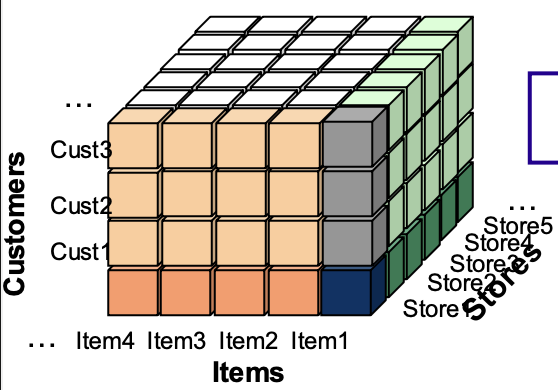
\includegraphics[width=\linewidth]{images/7-1.png}
    \end{minipage}
    \vspace{0.5em}
\end{definition}

\begin{theorem}
    {Cube operator}

    To compute a $n$ dimensional data cube, we need to compute $2^n$ group-bys to cover all combinations of dimensions.

    Example: For 3 dimensions (A, B, C), we need to compute group-bys for all of the following combinations:
    \begin{itemize}
        \item (A, B, C)
        \item (A, B), (A, C), (B, C)
        \item (A), (B), (C)
        \item ()
    \end{itemize}

    Adding \texttt{with cube} to a group-by statement computes all possible aggregations for the specified dimensions.

    Example:
    \begin{lstlisting}[language=SQL]
select a, b, c, aggr(d)
from ...
group by a, b, c with cube
\end{lstlisting}
\end{theorem}

\begin{theorem}
    {Cube size}
    For $n$ dimensions where each dimension $i$ has $d_i$ distinct values, the size of the data cube is given by (\textit{in tuples}):
    \[\text{Cube Size} = \prod_{i=1}^{n} (d_i + 1) = (d_1 + 1)(d_2 + 1) \cdots (d_n + 1)\]
    The "+1" accounts for the "ALL" value in each dimension.

    A \textbf{dense cube} has most cells ($> p\%$) filled with data, while a \textbf{sparse cube} has many empty cells.

    \[\text{Sparse cube size} \approx sf \times \text{Dense cube size}\]

    Where $sf$ is the sparsity factor.
\end{theorem}

\subsection{Materialization}

\textbf{Materialization} is the process of pre-computing and storing the results of data cube aggregations to improve query performance.

\begin{definition}
    {Benefit}
    For:
    \begin{itemize}
        \item \texttt{cma(view)} is the closest materialized ancestor
        \item \texttt{SV(view)} is the set of view of the view's subtree \textbf{including itself}
    \end{itemize}

    The benefit $B$ of materializing a view is:

    \begin{center}
        \texttt{(size(cma(view)) - size(view)) * count(SV(view))}
    \end{center}

    If view nodes have \textbf{workload distribution} \texttt{wl(v)}, the benefit formula becomes:

    \begin{center}
        \texttt{(size(cma(view)) - size(view)) * (sum(wl(v)) $\forall$ v $\in$ SV(view))}
    \end{center}
\end{definition}

\begin{theorem}
    {HRU Algorithm: Choosing views to materialize}

    \begin{itemize}
        \item Assuming root view a is already materialized.
        \item Numbers on view nodes are their sizes.
        \item To choose the next view to materialize, create a benefit column. Fill in all rows where the view is not yet materialized based on the benefit formula.
    \end{itemize}

    \tcblower


    \begin{minipage}{0.65\textwidth}
        Example:

        \begin{tabular}{l|l|l|l}
            View & Benefit (1st)                                & Benefit (2nd)                            & ... \\
            \hline
            b    & \colorbox{yellow}{$(100-50) \times 6 = 300$} & - (materialized)                         & ... \\
            c    & $(100-75) \times 6 = 150$                    & $(100-75) \times 2= 50$                  & ... \\
            d    & $(100-20) \times 3 = 240$                    & $(50-20) \times 3= 90$                   & ... \\
            e    & $(100-30) \times 4 = 280$                    & $(50-30) \times 4= 80$                   & ... \\
            f    & $(100-40) \times 3 = 180$                    & $(100-40) \times 1= 60$                  & ... \\
            g    & $(100-1) \times 2 = 198$                     & \colorbox{yellow}{$(50-1) \times 2= 98$} & ... \\
            h    & $(100-10) \times 2 = 180$                    & $(50-10) \times 2= 80$                   & ... \\
            i    & $(100-1) \times 1 = 99$                      & $(50-1) \times 1= 49$                    & ... \\
        \end{tabular}
    \end{minipage}
    \hfill
    \begin{minipage}{0.3\textwidth}
        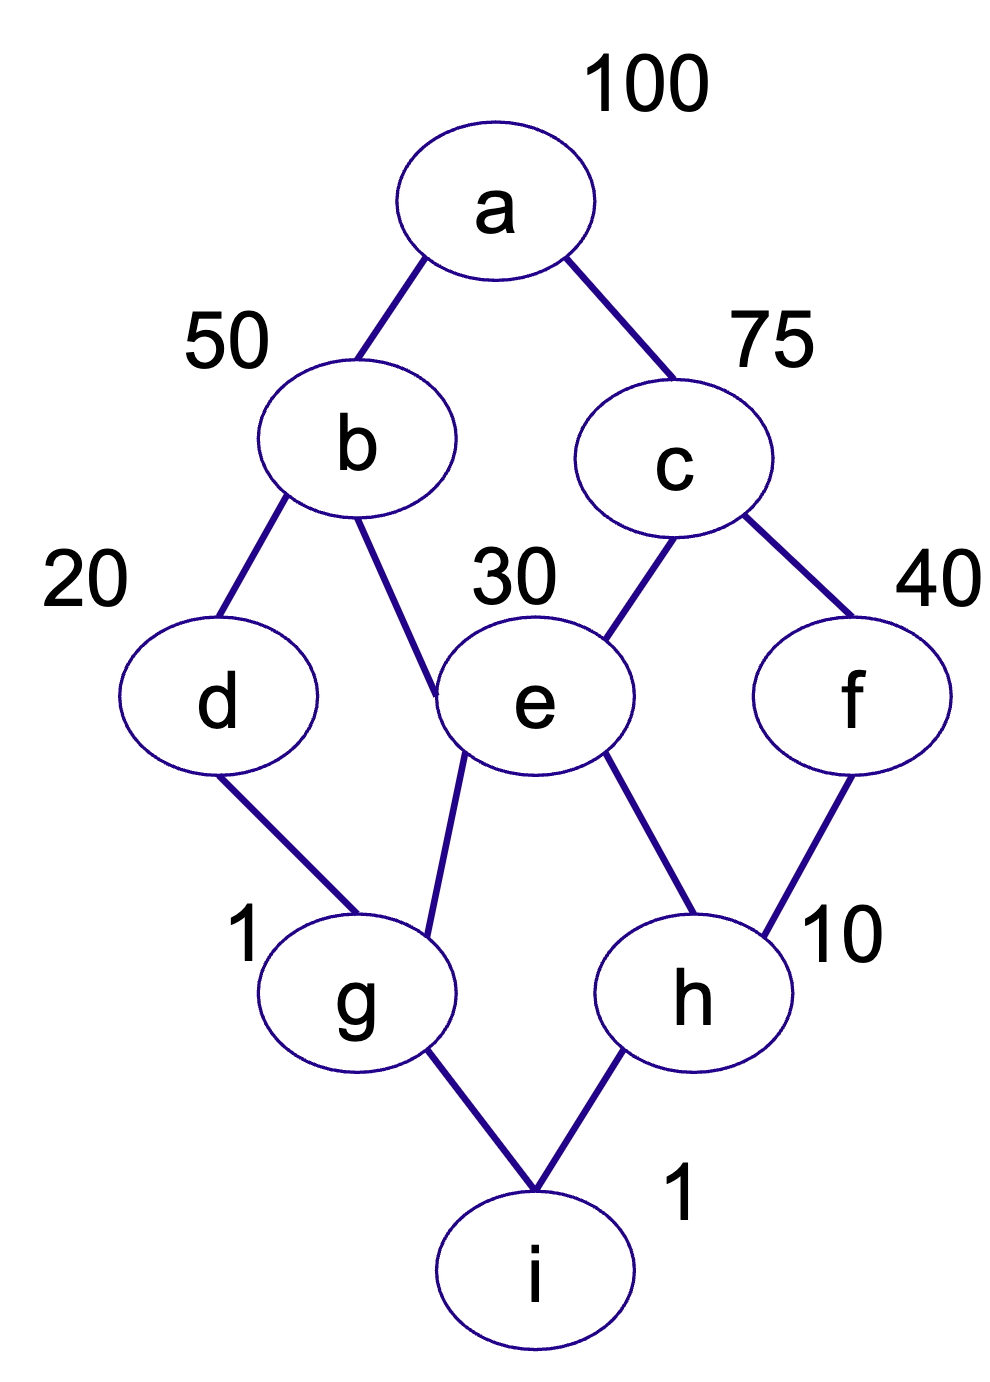
\includegraphics[width=\linewidth]{images/7-2.png}
    \end{minipage}

\end{theorem}
